\documentclass[12pt,a4paper]{report} % 使用report类,支持章节,12pt字号,A4纸
\usepackage[UTF8]{ctex} % 支持中文
\usepackage{graphicx} % 插入图片
\usepackage{hyperref} % 超链接
\usepackage{amsmath} % 数学公式
\usepackage{natbib} % 参考文献

% --- 页眉页脚(可选)---
% \usepackage{fancyhdr}
% \pagestyle{fancy}
% \fancyhf{}
% \fancyhead[L]{实验报告}
% \fancyhead[R]{\leftmark} % 显示当前章节
% \fancyfoot[C]{\thepage}

\title{LaTeX报告}
\author{刘浩洋 24040021022}
\date{2025年9月1日}

\begin{document}

% --- 前言部分 ---
\frontmatter % 前言部分,页码用罗马数字
\maketitle

% --- 摘要 ---
\begin{abstract}
本报告系统地介绍了使用LaTeX排版系统进行学术报告撰写的全过程。报告涵盖了从文档结构、字体、段落到数学公式、图表、参考文献等核心功能。通过多个实例,展示了LaTeX在科技文档排版中的强大能力与精确控制。结果表明,LaTeX是撰写高质量、专业级学术报告的理想工具。
\end{abstract}

% --- 目录 ---
\tableofcontents % 生成目录

% --- 正文部分 ---
\mainmatter % 正文部分,页码用阿拉伯数字,从1重新开始
\chapter{引言}
LaTeX是一种基于TeX的高质量排版系统,特别适用于科技和学术文档的撰写。与Word等所见即所得的编辑器不同,LaTeX采用标记语言,将内容与格式分离,从而让作者更专注于内容本身。

\section{研究背景}
随着学术交流的日益频繁,对文档格式的规范性和专业性要求越来越高。LaTeX因其卓越的排版质量,尤其是在数学公式和参考文献管理方面的优势,已成为学术界的事实标准。

\section{研究目标}
本报告旨在通过一系列实例,全面演示LaTeX在撰写报告时的核心功能,包括文本格式化、结构组织、数学公式输入、图表插入和文献引用等。

\chapter{LaTeX基础功能演示}
本章将通过具体实例展示LaTeX的基本用法。

\section{文本与段落}
LaTeX提供了丰富的命令来控制文本的字体、大小和颜色。例如,\textbf{粗体}、\textit{斜体}和\texttt{等宽字体}。段落首行默认缩进,可通过\texttt{\textbackslash parindent}调整。

\section{数学公式}
LaTeX的数学模式功能强大。例如,行内公式 $E = mc^2$,独立公式:
\[
\int_{-\infty}^{\infty} e^{-x^2} dx = \sqrt{\pi}
\]

\section{图表}
使用\texttt{figure}环境可以插入图片,如图\ref{fig:example}所示。
\begin{figure}[htbp]
    \centering
    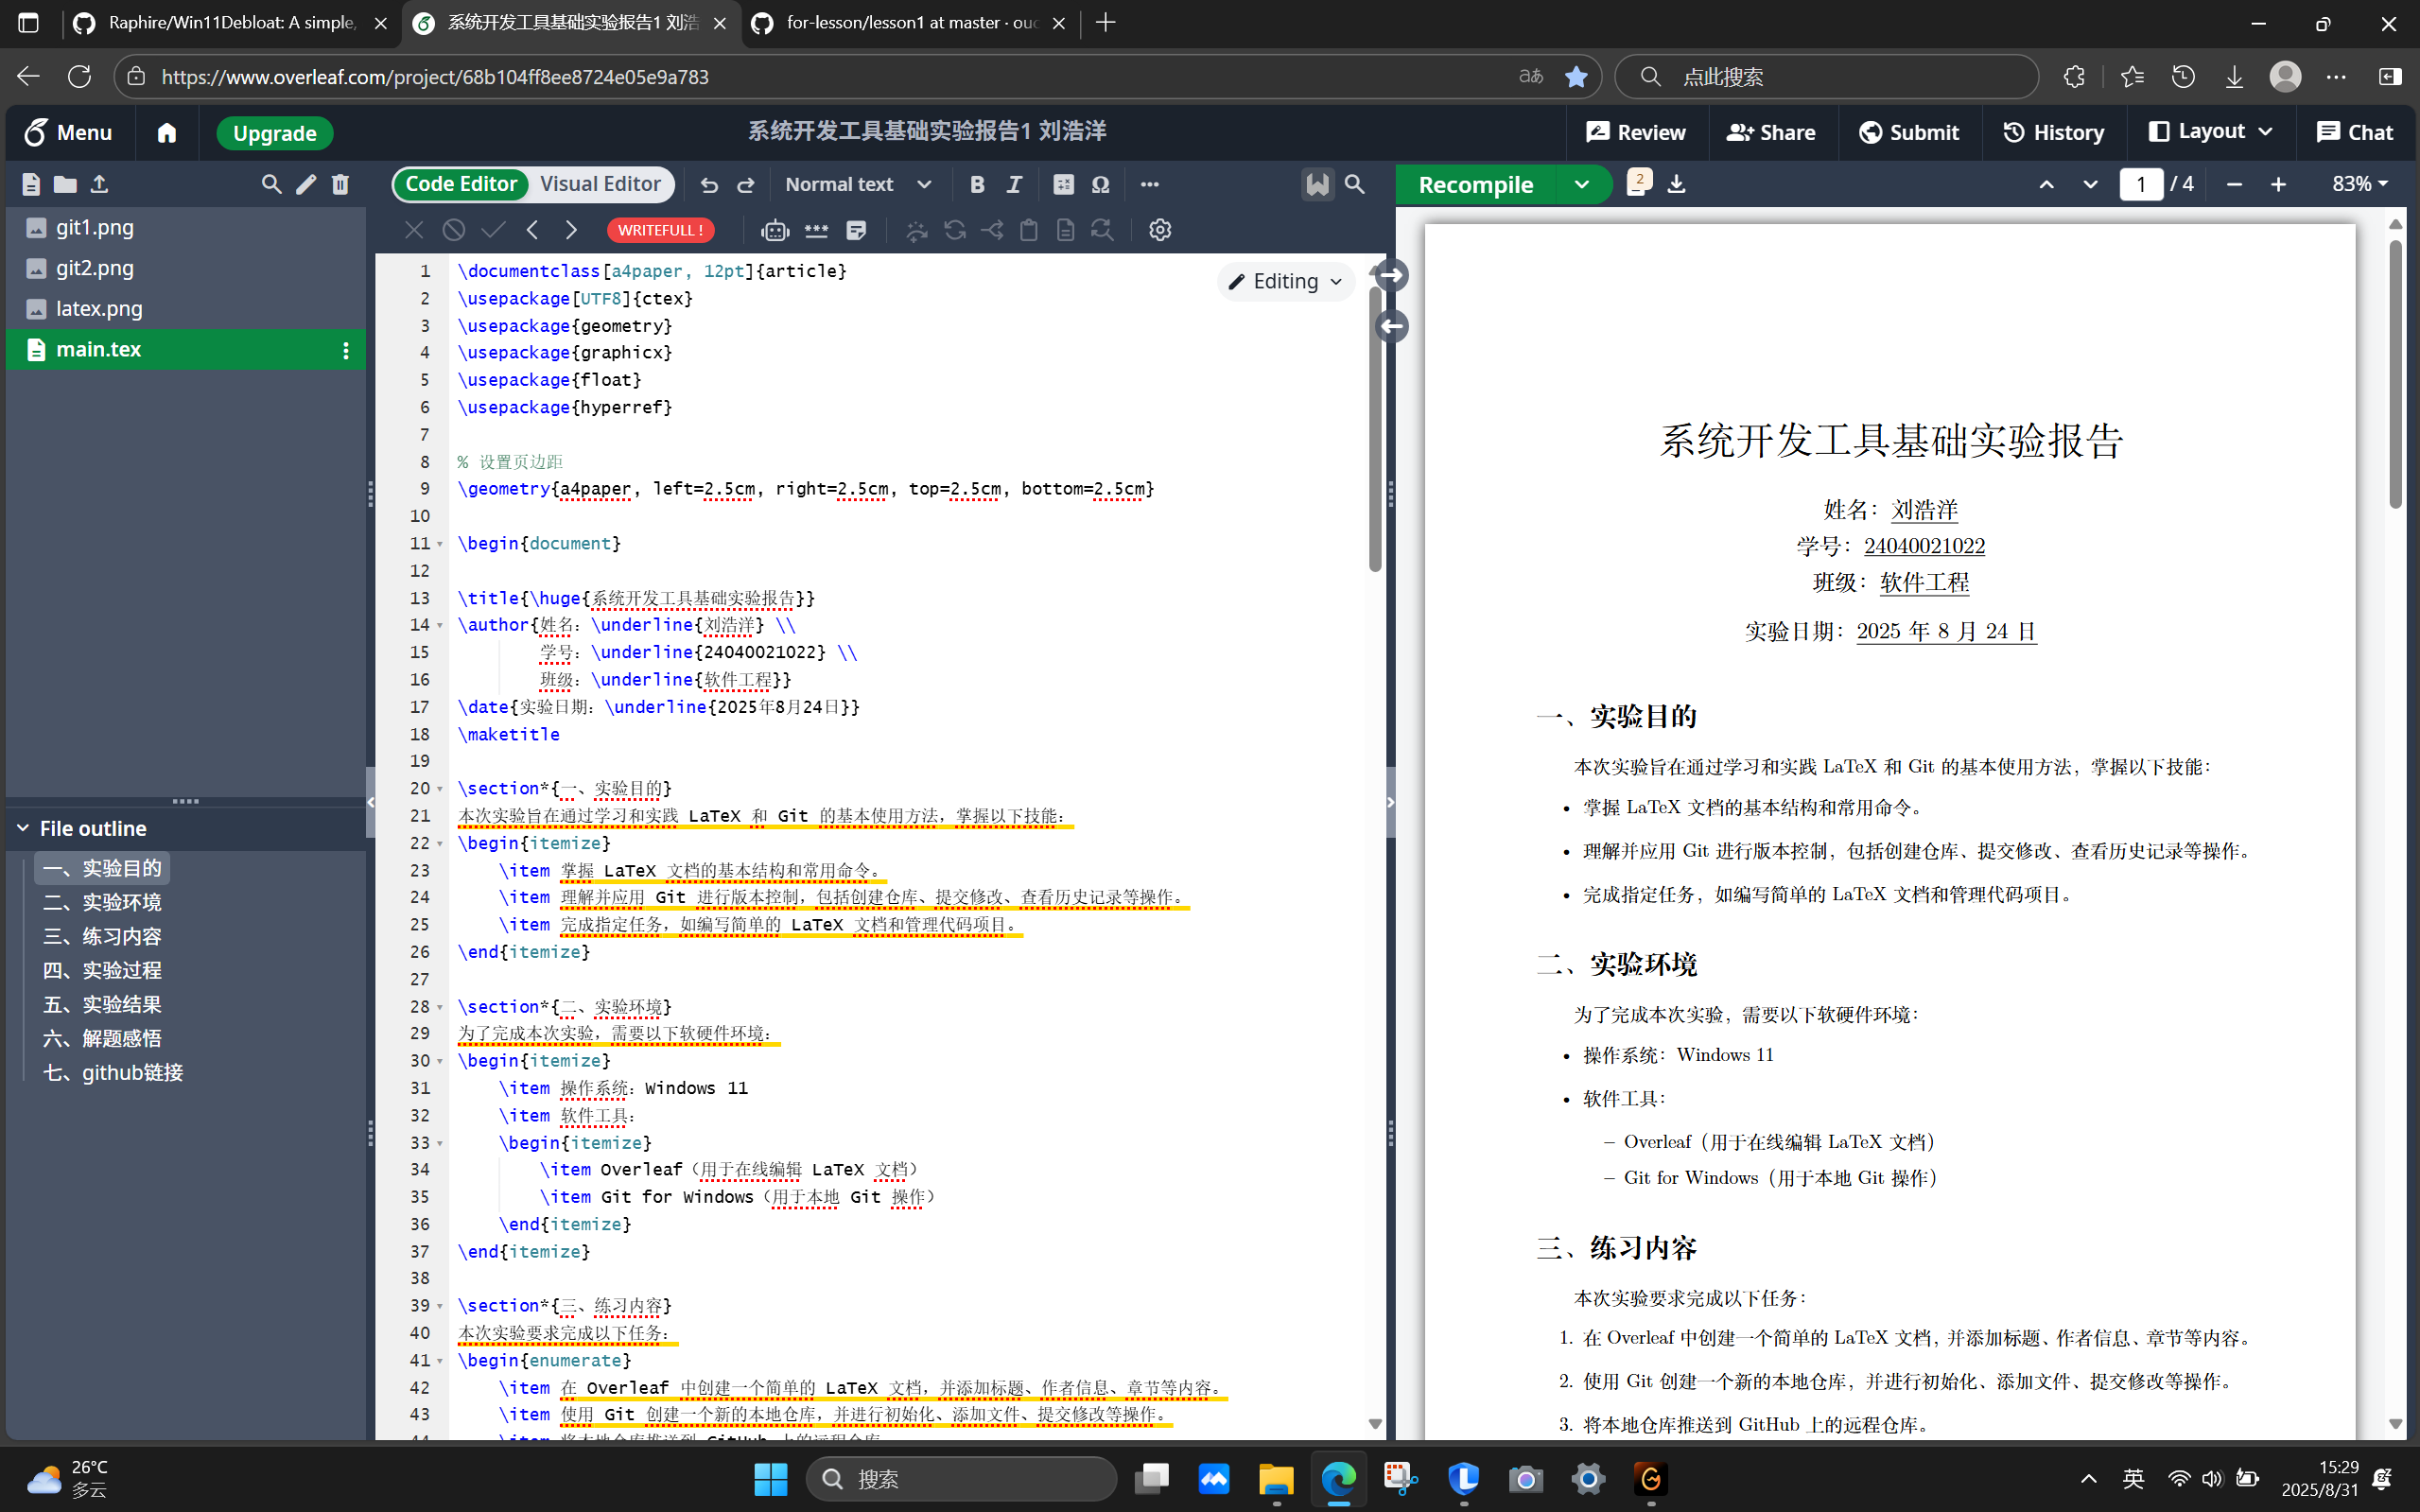
\includegraphics[width=0.5\textwidth]{example-image} % 使用Overleaf示例图片
    \caption{一个示例图片}
    \label{fig:example}
\end{figure}

\chapter{参考文献管理}
使用BibTeX可以高效管理参考文献。

\section{引用与标注}
在正文中通过\texttt{\textbackslash cite}命令引用文献,如Knuth的工作\cite{knuth1984}。

\section{参考文献列表}
\label{sec:ref}
\bibliographystyle{plain}
\bibliography{references} % 使用与之前实例相同的references.bib

% --- 附录部分 ---
\appendix % 开始附录
\chapter{附录A:LaTeX常用命令速查}
\begin{itemize}
    \item \texttt{\textbackslash textbf\{...\}}: 粗体
    \item \texttt{\textbackslash textit\{...\}}: 斜体
    \item \texttt{\textbackslash includegraphics\{...\}}: 插入图片
    \item \texttt{\textbackslash cite\{...\}}: 引用文献
\end{itemize}

% --- 后记部分 ---
\backmatter % 后记部分(通常无页码或特殊格式)
% 可以添加索引、致谢等

\end{document}